% Begin the document and set up the style of the document
\documentclass[a4paper]{article}

% Install the required packages for the document 
\usepackage{envmath}
\usepackage{esvect}
\usepackage{graphicx}
\usepackage{gensymb}
\usepackage{tikz}
\usepackage{geometry}
\usepackage{enumitem}
\usepackage{mathtools}
\usepackage{graphicx}
\usepackage{amsmath}
\usepackage{amscd}
\usepackage{amssymb}
\usepackage{amsfonts}
\usepackage{pgf,tikz}
\usepackage{mathrsfs}
\usepackage{asyalign}
\usepackage{cite}
\usepackage{url}
\usepackage[tableposition=top]{caption}
\usepackage{ifthen}
\usepackage[utf8]{inputenc}
\usetikzlibrary{arrows}





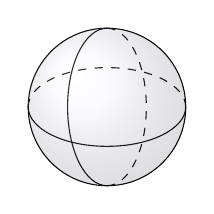
\begin{tikzpicture}
    \draw (-1,0) arc (180:360:1cm and 0.5cm);
    \draw[dashed] (-1,0) arc (180:0:1cm and 0.5cm);
    \draw (0,1) arc (90:270:0.5cm and 1cm);
    \draw[dashed] (0,1) arc (90:-90:0.5cm and 1cm);
    \draw (0,0) circle (1cm);
    \shade[ball color=blue!10!white,opacity=0.20] (0,0) circle (1cm);
\end{tikzpicture}
